\cotefile{29}
\scanpage{173}
Plan

% archive sheet number: 172

\scanpage{174}
\uline{Groupe fondamental}

I \deleted{\uline{Th. de comparaison} \unsure{pour un}} \inserted{Premier th. de \unsure{changemt|changement} de base pour $\pi_1$} (ou th. de comparaison)

II Deuxième th. de \unsure{changemt|changement} de base pour $\pi_1$

1) Morphismes $(-1)$-connexes et $0$-connexes

2) Morphismes locaux $(-1)$-connexes et $0$-connexes.

3) \deleted{Une} Caractérisation des morphismes locaux ou globaux $i$-connexes $(i=0,1)$.

4) \unsure{Les|Le} deux théorèmes de \deleted{comparaison} \inserted{\unsure{changemt|changement|chgt} de base pour $\pi_1$ :} énoncés et corollaires ...

5) \deleted{\unsure{Lemmes}, et} \deleted{\unsure{d}}Démonstration du théorème.

6) Généralisation à l'aide de la résolution des singularités.

7) Application à la dimension \unsure{cohomologique|chomologique} \unsure{des|de} certains corps ....

% archive sheet number: 173

\scanpage{175}
$\pi_2$

% archive sheet number: 174

\scanpage{176}
\diagram{\begin{tikzcd}[ampersand replacement=\&,column sep=3em,row sep=1.25em,
execute at end picture={\draw (xt.west) to[bend right=32] node[left] {$\widetilde{\pi}$} (xb.west);
\draw (xm.east) to[bend left=25] node[right] {$\widehat{\widetilde{\pi}}=\pi$} (xb.east);}]
|[alias=xt]| \unsure{\widetilde{\widetilde X}^{h}|\widehat{\widetilde X}^{h}|\widetilde{\widetilde X}^{i}}\arrow[d] \& \\
|[alias=xm]| \widetilde X^{h}\arrow[d] \& \widetilde X\arrow[d,no head]\\
|[alias=xb]| X^{h}\arrow[r] \& X
\end{tikzcd}}

\[
\begin{aligned}
\pi^{\mathrm{I}}(X,G)&\simeq H^{1}(\widetilde X,G)\simeq\underline{\lim}\,H^2(X_i,\unsure{G|C})\\
&\simeq\varinjlim H^2(\widetilde X_i,G)
\end{aligned}
\]

\margin{$\widetilde{\pi}/H_i=\pi_i$}

\[
H^*(\widetilde X_j,G)\Longleftarrow E^{pq}_2=H^p(H_i,H^q(\widetilde X,G))
\]
\[
\deleted{\unsure{H}}\pi^*(\widetilde X_j,G)\Longleftarrow E^{pq}_{\unsure{2}}=\varinjlim_i H^p(H_i,H^q(\widetilde X,G))
\]

\figure{\begin{tikzpicture}[x=.52cm,y=.43cm]
\draw (0,4.7) node[above left] {$q$} -- (0,0) -- (4.5,0);
\node at (6.1,-.5) {$p$};
\fill (0,0) circle (2pt); \draw[very thick] (1,0) circle (1.6pt);
\fill (2,0) circle (1.8pt); \fill (2.8,0) circle (1.8pt);
\node at (0,1) {$\times$}; \node at (1.1,1) {$\unsure{\times|\sim}$}; \node at (2,1) {$\times$};
\fill (0,2) circle (1.8pt); \fill (1,2) circle (1.6pt); \fill (2.2,2) circle (1.8pt);
\node at (5,3.5) {$\deleted{E^p}$};
\end{tikzpicture}}

\diagram{\begin{tikzcd}[ampersand replacement=\&,column sep=.8em,row sep=1.2em,
execute at end picture={
\draw (c.north east) to[out=150,in=90] (c.west) to[out=-90,in=220] (c.south east) to[out=40,in=-10] (c.north east);
\draw (e.north east) to[out=160,in=85] (e.west) to[out=255,in=190] (z.south east);
\draw ([xshift=-4pt]a.north west) to[out=-90,in=180] ([yshift=-4pt]b.south) -- (z.south east);}]
|[alias=a]| \scriptstyle\unsure{\cdot|0|\cdots}\arrow[r,no head] \&
|[alias=c]| \scriptstyle\varinjlim H^2(H_i,G)\arrow[r] \&
\scriptstyle\pi^2(X,G)\arrow[r] \&
\scriptstyle\varinjlim_i\pi^2(\deleted{\unsure{\widetilde X}}\unsure{X_i^h|X^h_i|\widetilde X_i},G)^{H_i}\arrow[r]\arrow[d,equal] \&
|[alias=e]| \scriptstyle\varinjlim H^3(H_i,G)\arrow[d]\\
\& |[alias=b]| {} \& {} \& \scriptstyle\pi^2(X^h,G) \& |[alias=z]| \scriptstyle H^{\unsure{3|2}}(\widetilde X,G)
\end{tikzcd}}

\[
\pi_2(X)\longrightarrow G
\]

\[
H^*(X^h,G)\Longleftarrow H
\]

\[
\operatorname{Ker}\bigl(\pi^2(X,G)\to\pi^2(X^h,G)\bigr)\simeq\varinjlim_i H^2(H_i,G)
\]
\[
\begin{aligned}
\operatorname{Coker}(\qquad\mathrm{id}\qquad)&\simeq\operatorname{Ker}\Bigl[\varinjlim H^3(H_i,G)\\
&\hspace{4em}\longrightarrow H^3(\widetilde X,G)\Bigr]
\end{aligned}
\]

% archive sheet number: 175

\scanpage{177}
\diagram{\begin{tikzcd}[ampersand replacement=\&,column sep=1.7em,row sep=1.2em]
\& Z' \& Z''_1\simeq{}Z''_2 \& \\
X\arrow[d] \& X'\arrow[l]\arrow[d] \& X''\arrow[l,shift left=.6ex]\arrow[l,shift right=.6ex]\arrow[d] \& \\
Y \& Y'\arrow[l]\arrow[d,equal] \& Y''\arrow[l,shift left=.6ex]\arrow[l,shift right=.6ex] \& \\
\& X \& \deleted{\widetilde Y''} \& \widetilde Y''\arrow[ul]
\end{tikzcd}}

\diagram{\begin{tikzcd}[ampersand replacement=\&,row sep=1.3em,column sep=1em]
\pi_1(\overline F)\arrow[r]\arrow[dr] \& \pi_1(X)\arrow[r]\arrow[d,dotted] \& \pi_1(Y)\arrow[r] \& e\\
\&G\&\&
\end{tikzcd}}
\[
\pi_1(Y)\longrightarrow G^{\pi_1(X)}
\]

\diagram{\begin{tikzcd}[ampersand replacement=\&,column sep=1.3em]
H^1(\pi_1(X),G)\arrow[r] \& H^1(\pi_1(\overline F),G)^{\pi_1(Y)}\\
H^1(\pi_1(Y),G^{\pi_1(\overline F)})=H^1(\pi_{\deleted{\unsure{1}}1}(Y),\unsure{z|\mathscr Z|\mathfrak{z}})\arrow[u] \&
\end{tikzcd}}

\[
\pi_1(Y)\longrightarrow z
\]
\[
H^1(\pi_1(\overline F),G)
\]
\[
\pi_1(Y')\longrightarrow z
\]
\[
H^1\bigl(Y'/Y,\operatorname{Hom}\bigl(\overset{\deleted{H^1}}{\overbrace{\pi_1(\overline F)}},z\bigr)\bigr)=0
\]

\diagram{\begin{tikzcd}[ampersand replacement=\&,column sep=1em]
\pi_1(Y) \& \pi_1(Y')\arrow[l,dashed] \& \pi_1(Y'')\arrow[l,shift left=.6ex]\arrow[l,shift right=.6ex]\arrow[dr] \& \pi_1(Y''')\arrow[l,shift left=1.1ex,dashed]\arrow[l,dashed]\arrow[l,shift right=1.1ex]\\
\&\&\&z
\end{tikzcd}}

% archive sheet number: 176

\scanpage{178}
$\pi_0,\pi_1$ \uline{et formalisme simplicial}

(Revêtements infinis)

% archive sheet number: 177

\scanpage{179}
\uline{Proposition} \quad $S$ un préschéma \uline{connexe},

$S'$ un préschéma sur $S$ tel que $S'\longrightarrow S$ soit \uline{submersif} [p. ex. fid$^{t}$ plat et quasi-compact, ou propre surjectif].

$S'',S'''$ les \unsure{carré|carrés}, cube fibré.

On suppose que $S'$ est \uline{somme} de \uline{préschémas} \uline{connexes} (i.e ses composantes connexes sont ouvertes, i.e. $\pi_0(S')$ discret), \deleted{et l'ens des composantes connexes de $S''$ \unsure{compac}}

Soit $\xi$ un pt [géométrique] de $S$. Alors pour un groupe discret $G$ variable, le foncteur
\[
G\leadsto\pi^1(S'/S,\xi\,;G)
\]
\deleted{\unsure{contrav|contravariant}} [où $\pi^1(S'/S,\xi\,;G)$ désigne l'ens des classes, à isom près, de données de descente sur \inserted{le fibré principal trivial} $G_{S'}$ relativement à $S'\to S$, pointées sur $\xi$] est strict.$^{t}$ proreprésentable :
\[
\pi^1(S'/S,\xi\,;G)=\varinjlim\operatorname{Hom}(\pi_i,G)
\]

Si $\pi_0(S'')$ est \inserted{quasi-}\uline{compact}, i.e. \unsure{tte|les} fonction loc constante sur $\pi_0(S'')$ n'a qu'un nb fini de valeurs, -- p. ex. $S''$ quasi-compact], \deleted{\unsure{ou} $S''$ n'a qu'un nb fini de composantes connexes]} \uline{alors} les $\pi_i$ sont de type fini. Si $S''$ a un nb fini \inserted{$n''$} de composantes connexes, alors le foncteur précédent est représentable : \deleted{de \unsure{façon}}
\[
\deleted{\text{\unsure{par}}}\pi^1(S'/S,\xi\,;G)\simeq\operatorname{Hom}(\pi_1(S'/S,\xi),G)
\]
avec $\pi_1(S'/S,\xi)$ \deleted{\unsure{engendré}} \inserted{\unsure{gpe|groupe} discret} de type fini. De façon précise, \deleted{\unsure{si}} le nb $n'$ des comp. conn. de $S'$ est alors fini, et $\deleted{n''-n'}\pi_1(S'/S;\xi)$ est engendré par $n''-n'$ générateurs.

% archive sheet number: 178

\scanpage{180}
\uline{Enfin}, considérons le \deleted{\unsure{--}}sous-foncteur
\[
G\leadsto\pi^1_{\mathrm{eff}}(S'/S,\xi\,;G)
\]
correspondant aux données de descente \uline{effectives} pointées sur $\xi$. \deleted{Ce \unsure{sera de} $\pi_0$} Ce foncteur est également \inserted{(\unsure{strictemt|strictement})} proreprésentable [par un système projectif de quotients des $\pi_i$].

\uline{N.B.} J'ignore, $\overline{\sim}$ si $S,S',S''$ noethériens, si ce dernier foncteur est $\overline{\sim}$ \uline{représentable}, à fortiori (comme $\pi^1(S'/S,\xi\,;G)$ est repr. dans ce cas) j'ignore si dans ce cas $\pi^1=\pi^1_{\mathrm{eff}}$, i.e. tte donnée de descente sur $G_{S'}$ rel : $S'/S$ est effective.
% slanted
\margin{Pb \unsure{résolu|résolue|intér.} \unsure{par|pour} l'affirmative [sous seule réserve \uline{$S$ \inserted{loc} noeth} \deleted{\unsure{]}} et $S'\to S$ fid plat quasi-compact]}
C'est vrai cependant [\unsure{ss|sans} hypothèse sur $S''$, $S$ et $S'$ étant loc noeth] si \deleted{\unsure{$G$ est}} dans $G$, $e$ est intersection de ss-groupes d'indice fini .....

% archive sheet number: 179

\scanpage{181}
\diagram{\begin{tikzcd}[ampersand replacement=\&,column sep=1.5em,row sep=1em]
Y \& X_0^{\deleted{0}}\arrow[l,dashed] \& X_1^{\deleted{1}}\arrow[l,shift left=.5ex]\arrow[l,shift right=.5ex] \& X_2^{\deleted{2}}\arrow[l,shift left=1ex]\arrow[l]\arrow[l,shift right=1ex]\\
\xi\arrow[u] \& X_{0\xi}^{\deleted{\unsure{0|\xi}}}\arrow[l]\arrow[u] \& X_{1\xi}^{\deleted{\unsure{1|\xi}}}\arrow[l,shift left=.5ex]\arrow[l,shift right=.5ex]\arrow[u] \& X_{2\xi}^{\deleted{2}}\arrow[l,shift left=1ex]\arrow[l]\arrow[l,shift right=1ex]\arrow[u]
\end{tikzcd}}

\diagram{\begin{tikzcd}[ampersand replacement=\&,column sep=1.5em,row sep=1.2em]
\& K_0^{\deleted{0}} \& K_1^{\deleted{1}}\arrow[l,shift left=.5ex]\arrow[l,shift right=.5ex] \& K_2^{\deleted{2}}\arrow[l,shift left=1ex]\arrow[l]\arrow[l,shift right=1ex] \& K_i^{\deleted{\unsure{i|\xi}}}=\pi_0(X_i^{\deleted{\unsure{i|\xi}}})\\
\unsure{\pi|\mathrm{T}} \& k_0^{\deleted{0}}\arrow[u,"i_0"] \& k_1^{\deleted{1}}\arrow[u,"i_1"]\arrow[l,shift left=.5ex]\arrow[l,shift right=.5ex] \& k_2^{\deleted{2}}\arrow[u,"i_2"]\arrow[l,shift left=1ex]\arrow[l]\arrow[l,shift right=1ex] \&
\end{tikzcd}}

\diagram{\begin{tikzcd}[ampersand replacement=\&,column sep=.5em,row sep=1.5em]
\pi_0(K) \& {}=\begin{gathered}\text{espace [compact ?]. associé au \unsure{treillis} des parties}\\ \text{ouvertes et fermées stables de } K^0=e\end{gathered}\\
\pi_0(k)\arrow[u] \& {}=\qquad\text{''}\qquad k^0=e
\end{tikzcd}}

Données de descente sur $E_{X^{\deleted{0}}_0}$ $\simeq$ Donnée de descente sur $E_{K^{\unsure{0}}}$ \deleted{\unsure{rel :|relatives}} (....)

$\simeq$ application continue $f:K_1^{\deleted{1}}\longrightarrow G$ telle que
\[
f(p'_1(\deleted{\unsure{1}}\xi_2))=f(p'_0(\xi_2))f(p'_2(\unsure{\xi_2|\xi_1|q_1}))\quad\text{pour }\forall\,\xi_2\in K .
\]

\uline{Équivalence} de telles :
\[
h(p_1(\xi))f(\xi)h(p_0(\unsure{y|\xi|q_1}))^{-1}\simeq f(y)
\]

Donnée de descente \deleted{\unsure{ponctuelle}} ponctuée sur $E_{X_0}$ $\simeq$ Donnée de descente ponctuée \inserted{(rel.$^{t}$ à $k^{\deleted{\unsure{2}}}_2$)} sur $E_{K^{\deleted{0}}_0}$

$\simeq$ application continue $f:K_1\unsure{\mathbin{-}|\to}G$ telle que
\[
\left\{\begin{aligned}
&f(i_1(\unsure{\eta_1|\xi_1|q}))=\deleted{\unsure{1_K|1}}e_G\quad\text{pour }\forall\,\eta_1\unsure{\in|\vdash} k_1\\
&\deleted{f(p'_1(y))=f}\quad f\circ p'_1=(f\circ p'_0)(f\circ p'_2)
\end{aligned}\right.
\]

Équivalence de telles : \deleted{\unsure{un}}
\[
h(p_1(y))f(y)h(p_0(y))^{-1}\simeq f(y)
\]
Si \quad $h(i_0(y_0))=1\quad\forall\,i_0$

% archive sheet number: 180

\scanpage{182}
Pratiq$^{\mathrm{mt}}$, \unsure{cel.|cela|on} revient à contracter $i_0(k_0),i_1(k_1),i_2(k_2)$ en des pts, et \unsure{de} se borner à des \unsure{cochaines|cochaînes} normalisées sur \deleted{\unsure{le complexe}} \inserted{l'\unsure{espace|ensemble} simplicial} \uline{ponctué} obtenu
\diagram{\begin{tikzcd}[ampersand replacement=\&,column sep=1em]
\overline K_0 \& \overline K_1\arrow[l,shift left=.6ex]\arrow[l,shift right=.6ex] \& \overline K_2\arrow[l,shift left=1.1ex]\arrow[l]\arrow[l,shift right=1.1ex]
\end{tikzcd}}

On utilise le fait que
\[
\begin{aligned}
\pi_0(k_*)&=e\\
\text{``}\,\pi_1(k_*)&=e\,\text{''}\qquad\text{i.e. }\pi^1(k_*,G)=e
\end{aligned}
\]
\uline{donc tte donnée de descente admet une ponctuation}

et on utilisera le fait
\[
\pi_0(K_*)=e
\]
pour le fait que \deleted{deux ponctuations} tout \uline{automorphisme} d'une structure de descente \uline{ponctuée} est trivial. \deleted{[et \unsure{tt autom} d'une structure de descente, \unsure{pas néc.} ponctuée, est \unsure{définie|défini} par un élémt de $G$, \unsure{évidemt} unique]}

\deleted{Regardons les}

% archive sheet number: 181

\scanpage{183}
$\pi_0$

\figure{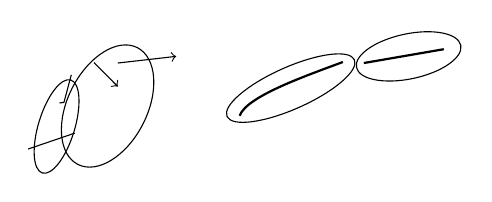
\begin{tikzpicture}[x=.72cm,y=.65cm]
\draw[thin,rotate around={-17:(.55,.65)}] (.55,.65) ellipse (.32 and .95);
\draw[thin,rotate around={-27:(1.45,1.05)}] (1.45,1.05) ellipse (.7 and 1.28);
\draw[thin] (.05,.21) -- (.87,.52);
\draw[thin] (.81,1.66) -- (.68,1.12) -- (.6,1.11);
\draw[->,thin] (1.21,1.9) -- (1.63,1.43);
\draw[thin,->] (1.63,1.89) -- (2.66,2.02);
\draw[rotate around={24:(4.68,1.4)}] (4.68,1.4) ellipse (1.23 and .41);
\draw[thick] (3.78,.86) .. controls (3.9,1.24) and (4.95,1.64) .. (5.6,1.91);
\draw[rotate around={12:(6.76,2.02)}] (6.76,2.02) ellipse (.94 and .44);
\draw[thick] (5.97,1.89) -- (7.38,2.16);
\end{tikzpicture}}

\diagram{\begin{tikzcd}[ampersand replacement=\&,column sep=1em]
F^0\arrow[r,shift left=.6ex]\arrow[r,shift right=.6ex]\& F^1\arrow[r,shift left=1.1ex]\arrow[r]\arrow[r,shift right=1.1ex]\&F^2
\end{tikzcd}}

foncteurs $(\mathrm{Ens})\to(\mathrm{Ens})$

objet simplicial de $\underline{\operatorname{Hom}}(\mathrm{Ens},\mathrm{Ens})$

Permet en principe de définir des $\pi_0,\pi_1$

$\pi_0(F)$, $F\in\underline{\operatorname{Hom}}(\mathrm{Ens},\mathrm{Ens})$, $F$

\[
F(I)\underset{?}{\simeq}C(K,I)\qquad K\ \text{espace top \uline{tot. discontinu}}
\]
[deux pts sont séparés par un ens : à la fois ouvert et fermé]

\uline{Cond néc} a) $F$ commute aux \deleted{\unsure{produits}} $\varprojlim$ finies i.e. $F$ \uline{exact à gauche} [donc $F$ transforme mon. en mon]

b) $F(\bigcap I_\alpha)=\bigcap_\alpha F(I_\alpha)$ pour \deleted{\unsure{(tous)|(toute)}} famille filtrante de sous-ens. de $I$

Ces conditions équivalent à : \uline{$F$ strictement proreprésentable} par un système projectif strict $(\pi_{0\,i})_i$ \deleted{\unsure{de}} d'ensemble.

Il faut de plus

c) $\deleted{\unsure{\pi_0=|\text{Alors}}}\varprojlim\pi_{0\,i}\longrightarrow\pi_{0\,i}$ est \uline{surjectif} pour $\forall\,i$

Ces conditions sont \uline{néc} et suffisantes, et on pourra prendre $K=\varprojlim\pi_{0\,i}$, avec la topologie limite inverse des top. discrètes. \uline{NB} \unsure{Si} $F$ est donné dans la forme $C(L,I)$, $L$ esp. top., alors $\pi_0(L)\longrightarrow K$. Si $L$ est \inserted{(quasi)} compact, cet hom est un isomorphisme ; \uline{en général}, ce n'est ni injectif, ni surjectif,

\margin{Bourb. Topologie \unsure{II|2} p. 232, prop. 6}

% archive sheet number: 182

\scanpage{184}
\deleted{\diagram{\begin{tikzcd}[ampersand replacement=\&,execute at end picture={
\begin{scope}[x=.01075cm,y=-.01075cm,>=stealth,every node/.style={font=\scriptsize,inner sep=.7pt},line width=.4pt]
\node at (294,80) {$\overline K_0\ \substack{\longleftarrow\\[-.45ex]\longleftarrow}\ \overline K_1\ \substack{\longleftarrow\\[-.45ex]\longleftarrow\\[-.45ex]\longleftarrow}\ \overline K_2$};
\draw[-] (195,105) -- (185,121);
\draw[-] (274,120) -- (305,152);
\draw[-] (371,120) -- (343,147);
\node at (182,136) {fini};
\node at (328,169) {\shortstack{\unsure{cpt|cpts|gpe} tot\\ \unsure{disco|disc|discret}}};
\node at (740,49) {$x$};
\node at (587,91) {$\mathbb Z$};
\node at (696,133) {$F$};
\node at (494,158) {$A$};
\node at (420,217) {$\deleted{f(x,y)}$};
\node at (514,238) {$\unsure{\Lambda|\wedge}$};
\node at (621,198) {$k[[s,t]]$};
\draw[-] (662,211) -- (674,214);
\node at (616,235) {$k$ \unsure{sép|alg.} clos};
\node at (878,165) {$\overline K_1\unsure{\to|\mathbin{-}}G$ opère sur $\unsure{E|\overline E|\overline F}$};
\node at (901,222) {de façon que $\overline K_1$ y \uline{opère}};
\node at (876,270) {\uline{\unsure{continûmt|continûment|continue}}};
\draw[-] (730,279) -- (767,236);
\fill (45,282) circle (.8pt);
\fill (113,284) circle (.8pt);
\fill (144,264) circle (.8pt);
\fill (179,264) circle (.8pt);
\fill (208,238) circle (.8pt);
\fill (227,266) circle (.8pt);
\fill (142,306) circle (.8pt);
\fill (183,307) circle (.8pt);
\fill (218,307) circle (.8pt);
\fill (174,235) circle (.8pt);
\fill (204,208) circle (.8pt);
\fill (211,201) circle (.8pt);
\draw[->] (45,282) -- (85,283);
\draw[->] (85,283) -- (114,284);
\draw[->] (115,283) -- (145,263);
\draw[->] (145,262) -- (177,234);
\draw[->] (177,232) -- (204,207);
\draw[->] (209,203) -- (235,171);
\draw[->] (210,202) -- (249,195);
\draw[->] (148,264) -- (180,264);
\draw[->] (187,262) -- (211,239);
\draw[->] (214,235) -- (239,213);
\draw[->] (213,238) -- (248,241);
\draw[->] (186,265) -- (228,266);
\draw[->] (229,265) -- (266,249);
\draw[->] (227,265) -- (271,275);
\draw[->] (116,284) -- (142,305);
\draw[->] (147,305) -- (185,305);
\draw[->] (187,305) -- (220,305);
\draw[->] (220,305) -- (255,306);
\draw[->] (219,308) -- (258,343);
\node at (460,298) {$g(p(\unsure{t_1|h_1}))\,f(t_1)\,g(q(t_1))^{-1}$};
\node at (460,356) {$\pi_1^{\mathrm{eff}}(S,a)$};
\node at (939,309) {$S$ connexe};
\node[draw,inner sep=1.4pt] at (939,351) {$\pi_1^{\mathrm{eff}}(S,a)$};
\fill (879,389) circle (.8pt);
\node at (879,419) {$\unsure{s|S}$};
\fill (819,404) circle (.8pt);
\node at (248,399) {$\overline E$};
\draw[-] (249,423) -- (253,466);
\fill (254,475) circle (.8pt);
\fill (332,404) circle (.8pt);
\draw (332,404) .. controls (355,409) and (376,383) .. (375,374);
\fill (118,439) circle (.8pt);
\fill (134,503) circle (.8pt);
\fill (282,501) circle (.8pt);
\fill (340,477) circle (.8pt);
\draw[->] (118,442) -- (39,558);
\draw[->] (39,565) -- (128,509);
\draw[->,thick] (136,498) .. controls (154,481) and (148,455) .. (132,438);
\draw[->] (285,501) -- (341,478);
\node at (285,515) {$x$};
\node at (347,489) {$a$};
\draw[->] (346,469) .. controls (395,420) and (353,395) .. (342,467);
\node at (373,423) {$'$};
\node at (144,568) {$\deleted{f(x,y)}$};
\node at (121,627) {$f(\unsure{u|w})$};
\draw[->] (433,509) -- (529,445);
\fill (535,441) circle (.8pt);
\draw[->] (536,435) -- (574,349);
\fill (580,334) circle (.8pt);
\node at (599,328) {$b$};
\draw[->] (598,460) -- (649,445);
\draw[->] (662,441) -- (688,423);
\draw[->] (692,419) -- (720,381);
\fill (722,381) circle (.8pt);
\draw[->] (723,361) -- (741,332);
\fill (741,332) circle (.8pt);
\draw[->] (756,325) -- (803,325);
\draw[->] (816,324) -- (849,331);
\draw[->] (731,377) -- (852,343);
\node at (601,498) {$S\leftarrow S'$};
\draw[->] (474,543) -- (514,526) .. controls (550,488) and (499,463) .. (478,518) .. controls (473,527) and (471,539) .. (477,535);
\fill (228,629) circle (.8pt);
\fill (299,609) circle (.8pt);
\draw[->] (227,629) -- (297,611);
\draw[->] (300,610) -- (350,577);
\draw[->] (353,578) -- (384,525);
\draw[->] (354,581) -- (406,581);
\draw[->] (402,574) -- (386,541);
\node at (268,584) {$u_1$};
\node at (193,675) {$K_1$};
\node at (302,666) {$K_1$};
\fill (420,659) circle (.8pt);
\draw[->] (419,659) -- (474,637);
\draw[->] (475,637) -- (501,606);
\fill (501,606) circle (.8pt);
\draw[->] (502,606) -- (559,609);
\draw[->] (564,609) -- (597,609);
\draw[->] (596,600) -- (595,549);
\node at (601,620) {$a$};
\draw[->] (356,739) .. controls (351,720) and (335,666) .. (368,644) .. controls (392,634) and (354,730) .. (348,682) -- (357,743);
\draw[->] (363,741) .. controls (383,700) and (401,618) .. (379,656) .. controls (354,694) and (381,752) .. (400,646) .. controls (416,666) and (382,727) .. (365,743);
\draw[->] (384,746) .. controls (406,699) and (445,656) .. (427,681) .. controls (404,665) and (375,721) .. (400,728) .. controls (417,728) and (430,677) .. (418,691) -- (383,748);
\node at (396,797) {$\deleted{\unsure{B}}A\leftarrow A'$};
\fill (197,770) circle (.8pt);
\draw[->] (197,770) -- (229,748) -- (260,769) -- (291,730);
\fill (519,728) circle (.8pt);
\node at (513,744) {$a_0$};
\draw[->] (535,728) -- (687,723);
\draw[->] (535,721) -- (675,655);
\draw[->] (689,717) .. controls (682,695) and (682,673) .. (685,659);
\node at (630,635) {$x$};
\fill (793,559) circle (.8pt);
\node at (800,578) {$a$};
\node at (856,467) {$b$};
\node at (760,429) {$\unsure{c|E}$};
\node at (751,511) {$d_1$};
\node at (816,445) {$d_2$};
\node at (849,526) {$d_0$};
\draw[->] (645,634) -- (777,563);
\draw[->] (646,628) -- (774,566);
\draw[->] (650,618) -- (741,468);
\draw[->] (740,459) -- (652,607);
\draw[->] (828,489) -- (667,614);
\draw[->] (653,608) -- (827,482);
\draw[->] (791,550) -- (763,448);
\draw[->] (808,555) -- (847,482);
\draw[->] (829,467) -- (778,450);
\draw[-] (800,457) -- (773,506);
\draw[-] (810,474) -- (791,513);
\draw[-] (821,482) -- (806,522);
\draw (782,495) -- (788,507) -- (796,501) -- (805,506);
\node at (741,694) {$x$};
\fill (767,684) circle (.8pt);
\draw[-] (747,704) -- (902,628);
\draw[->] (896,581) -- (767,685);
\draw[->] (921,615) -- (901,567);
\draw[->] (935,570) -- (979,550);
\draw[->] (969,539) -- (919,558);
\draw[->] (983,552) -- (995,504);
\draw[->] (975,505) -- (971,540);
\draw[->] (985,497) -- (1015,483);
\draw[->] (989,505) -- (1037,487);
\draw[->] (1036,484) -- (1046,432);
\draw[->] (1042,444) -- (1031,481);
\draw[->] (1040,480) -- (1049,434);
\draw[->] (935,580) .. controls (970,574) and (1006,535) .. (1005,508);
\node at (1060,427) {$a$};
\node at (873,729) {$x$};
\node at (1029,663) {$a$};
\draw[->] (882,717) -- (918,700);
\draw[->] (913,699) -- (880,710);
\draw[->] (931,704) -- (970,684);
\draw[->] (965,679) -- (932,695);
\draw[->] (977,676) -- (1016,656);
\draw[->] (1009,652) -- (974,670);
\draw[->] (656,791) -- (799,736);
\draw[->] (797,731) -- (653,786);
\node at (911,729) {$u_n$};
\node at (963,707) {$u_{n-1}$};
\node at (1009,682) {$u_1$};
\draw[thin] (113,100) -- (608,363) -- (1027,666);
\draw[thin] (656,68) .. controls (736,163) and (873,229) .. (1006,332);
\draw[thin] (89,343) .. controls (125,408) and (324,501) .. (452,612) .. controls (602,729) and (738,813) .. (783,813);
\end{scope}}]
\phantom{.}
\end{tikzcd}}}
% archive sheet number: 183

\scanpage{185}
mais il est naturel de mettre sur $\pi_0(L)$ la topologie image inverse de $K$. [topologie \inserted{des $\pi_0(L)$} des partitions ouvertes de $L$]. $F$ est dit \uline{connexe} si $F\simeq\mathrm{id}_{\mathrm{Ens}}$, i.e. $F$ est T-représentable par l'espace ponctuel [i.e. par un espace connexe].

Considérons deux \deleted{foncteurs} flèches
\diagram{\begin{tikzcd}[ampersand replacement=\&,column sep=1em]
F^*:\quad F^{\deleted{0}0}\arrow[r,shift left=.5ex]\arrow[r,shift right=.5ex]\&F^{\deleted{1}1}\qquad(F^0,F^1\in\underline{\operatorname{Hom}}(\mathrm{Ens},\mathrm{Ens}))
\end{tikzcd}}
et le \uline{foncteur noyau}
\[
\pi^0(F^*)=F=\operatorname{Ker}(F^0\rightrightarrows F^1)
\]

Si $F^0,F^1$ sont \deleted{\unsure{strictement pro|strictement}}\inserted{T-}représentables, alors les deux flèches proviennent de flèches
\diagram{\begin{tikzcd}[ampersand replacement=\&,column sep=1em]
K_0 \& K_1\arrow[l,shift left=.6ex]\arrow[l,shift right=.6ex]
\end{tikzcd}}
et $F$ sera \unsure{égalt|égalemt|également} T-représentable [N.B. Toute $\varprojlim$ de foncteurs T-représentables est T-repr, en prenant une limite inductive sur les espaces dont ils proviennent --, \deleted{\unsure{et}} et le $\pi_0$ associé]. Un \deleted{\unsure{couple}} $F^{\unsure{\alpha|*}}$ comme dessus est dit \uline{connexe} si son noyau est connexe.

Considérons un ``foncteur $\frac12$cosimplicial'', \unsure{ie|de} \inserted{objet $\frac12$\inserted{co}simplicial de} $\underline{\operatorname{Hom}}(\mathrm{Ens},\mathrm{Ens})$
\diagram{\begin{tikzcd}[ampersand replacement=\&,column sep=1em]
F^0\arrow[r,shift left=.6ex]\arrow[r,shift right=.6ex]\&F^1\arrow[r,shift left=1.1ex]\arrow[r]\arrow[r,shift right=1.1ex]\&F^2
\end{tikzcd}}
On lui associe foncteurs $\pi^0(F^*;E)$ et \deleted{\unsure{et|$\xi$}}, $\pi^1(F^*,G)$, où $E$ ens variable, $G$ groupe variable. Si $F^*$ est \uline{coponctué} i.e. muni de $F^*\to\mathrm{id}_{\mathrm{Ens}}^*$, on définit de $\overline{\sim}$ $\pi^0(F^*,\xi;E)$ et $\pi^1(F^*,\xi;G)$, $\xi$

% archive sheet number: 184

\scanpage{186}
désignant la ponctuation. Plus précisément, si on a un autre foncteur $\frac12$\inserted{co}simplicial
\diagram{\begin{tikzcd}[ampersand replacement=\&,column sep=1em]
f^0\arrow[r,shift left=.6ex]\arrow[r,shift right=.6ex]\&f^1\arrow[r,shift left=1.1ex]\arrow[r]\arrow[r,shift right=1.1ex]\&f^{\unsure{2|?}}
\end{tikzcd}}
\deleted{on va \unsure{se}} et un hom $\frac12$\inserted{co}simplicial $\xi$
\diagram{\begin{tikzcd}[ampersand replacement=\&,column sep=1em,row sep=1.4em]
\&F^0\arrow[r,shift left=.6ex]\arrow[r,shift right=.6ex]\arrow[d,"\xi^0"]\& F^1\arrow[r,shift left=1.1ex]\arrow[r]\arrow[r,shift right=1.1ex]\arrow[d,"\xi^1"]\&F^2\arrow[d,"\xi^2"]\\
\xi:\&f^0\arrow[r,shift left=.6ex]\arrow[r,shift right=.6ex]\&f^1\arrow[r,shift left=1.1ex]\arrow[r]\arrow[r,shift right=1.1ex]\&f^2
\end{tikzcd}}
on définit $\pi_0(F^*,\xi;E)$ et $\pi^{\unsure{2|1}}(F^*,\xi;E)$.

Si $F^0,F^1,F^2$ sont T-représentables, et dans le cas où on \unsure{se donne|les a un} \deleted{\unsure{de}} $\xi:F^*\unsure{\mathbin{-}|\to} f^*$, si $f^*$ est T-représentable, on ramène ceci à la donnée d'un \deleted{objet} \uline{espace $\frac12$simplicial}
\diagram{\begin{tikzcd}[ampersand replacement=\&,column sep=1em]
K_0\&K_1\arrow[l,shift left=.6ex]\arrow[l,shift right=.6ex]\&K_2\arrow[l,shift left=1.1ex]\arrow[l]\arrow[l,shift right=1.1ex]
\end{tikzcd}}
resp. d'un \uline{espace $\frac12$simplicial} \uuline{ponctué} (par contraction)
\diagram{\begin{tikzcd}[ampersand replacement=\&,column sep=1em]
\overline K_0\&\overline K_1\arrow[l,shift left=.6ex]\arrow[l,shift right=.6ex]\&\overline K_2\arrow[l,shift left=1.1ex]\arrow[l]\arrow[l,shift right=1.1ex]
\end{tikzcd}}
par un procédé \unsure{standard|standart} .....

Il y a lieu de généraliser ces constructions au cas où sur les $K_i$, resp. des $\overline K_i$, on a des catégories galoisiennes \unsure{attachées|étalées|itérées} à chaque pt, \deleted{(\unsure{ou encore}, les \unsure{pts|$F_\xi$}} pour décrire des relations de descente à la \uline{Van Kampen} .....

% archive sheet number: 185

\scanpage{187}
\uline{Proposition} \quad Soit $f:X\unsure{\mathbin{-}|\to}Y$ un morphisme, avec

\begin{tabular}{|p{.86\linewidth}}
1) \deleted{$f$ loc de présentation finie et \unsure{loc} quasi-fini} \inserted{$Y$ loc. noeth et \unsure{univ.} japonais}\\[.25em]
2) $\deleted{\unsure{f}}X$ \deleted{irréductible} n'a qu'un nb fini de comp. irréd.\\[.25em]
3) $f$ loc. \inserted{de type fini,} quasi-fini \deleted{et \unsure{sé}}, $f$ \uline{séparé}
\end{tabular}

\begin{tabular}{|p{.86\linewidth}}
Sous ces conditions, $f$ est \uline{de type fini}
\end{tabular}

$-$

On peut supposer $\deleted{\unsure{S|X}}Y$ affine donc noeth, \deleted{\unsure{$f$}} $X$ intègre, \deleted{et $f$ dominant} \inserted{(car il suffit de voir que $f$ est qu. \unsure{cpt|cqt})}. Soit $U$ un ouvert \inserted{affine} non vide de $X$, il est quasi-fini séparé sur $Y$, donc par le main theorem il est $Y$-isomorphe
\diagram{\begin{tikzcd}[ampersand replacement=\&,column sep=1.25em,row sep=.55em]
\& X''\arrow[dl,"\text{fini}"']\arrow[dd]\\
X\arrow[dd]\&\\
\& X'\arrow[dl,"\substack{\text{fini}\\\text{\unsure{surj}}}"]\\
Y\&
\end{tikzcd}}
à un ouvert d'un \deleted{\unsure{fini $X'$ de $Y$}} \inserted{$Y$-}préschéma \uline{fini} $X'$, qu'on peut supposer intègre. Soit $X''$ \unsure{le} sous-préschéma fermé intègre de $X\times_Y X'$ \deleted{\unsure{propre de} \illegible{1}} \inserted{adhérence de} la ``diagonale'' de $U\times_Y U'$, donc $X''$ s'envoie dans $X$ et $X'$. Alors $X''\to X$ est fini, et étant dominant, est \uline{surjectif}. Il suffit donc de voir que $X''$ est de t.f. sur $Y$, ou \unsure{même} sur $X'$. Or $X''\to X'$ est un morphisme birationnel, \unsure{avec|car} $X''$ et $X'$ intègres. Donc \deleted{\unsure{$X'$|il}}il y a un $X'$-morphisme \uline{surjectif} $\widetilde X'\to X''$, où $\widetilde X'$ est le normalisé. Or $\widetilde X'$ est fini sur $Y$, on gagne .....

% archive sheet number: 186
